
\section{Orthogonality Assumption}
\label{sec:orthogonality-assumption}

A key assumption in our theoretical results is that the features are orthogonal to one
another. In general, this is a strong assumption that is rarely satisfied in practice. In
the high-dimensional setting with binary data, it is even impossible to achieve. In spite
of this, it turns out that the assumption holds little bearing on our results.

The primary reason for this is a well-known behavior of regularized estimators when
features are correlated. Since information about the effect is shared between the
correlated features, the objective can attain a lower value by favoring one of the features
over the others. The effect is particularly strong in the lasso, which is known to select
only one of the correlated features and ignore the others given a sufficiently large
correlation and penalty strength.

A second reason for why the assumption is not as restrictive as it may seem is that the
correlation between two features, at least one being binary, tends to zero as class balance
increases towards one. We first demonstrate this empirically in the following experiment.
We consider a setting with two binary features: the first, \(\bm{x}_1\) with class balance
\(q_1 = 0.5\), and the second, \(\bm{x}_2\), with varying balance \(q_2 \in [0.5, 0.9]\).
We set the true effect to \(\beta_1^* = \beta_2^* = 1\) and the level of correlation,
\(\rho\) to three different levels (0, 0.4, and 0.6). The noise level
\(\sigma_\varepsilon\) is set to obtain a signal-to-noise ratio of 1. We generate
\(n=\num{10000}\) observations and fit the lasso with \(\lambda = \lambda_\text{max}/2\).

The results are shown in \Cref{fig:orthogonality} where we see that the effect of
correlation has no impact on the shrinkage imposed from decreasing class balance of the
second feature. The results in fact suggest that the effect of \(q_2\) is \emph{stronger}
when the features are correlated, which is due to the nature of the lasso that we
previously discussed.

\begin{figure}[htpb]
  \centering
  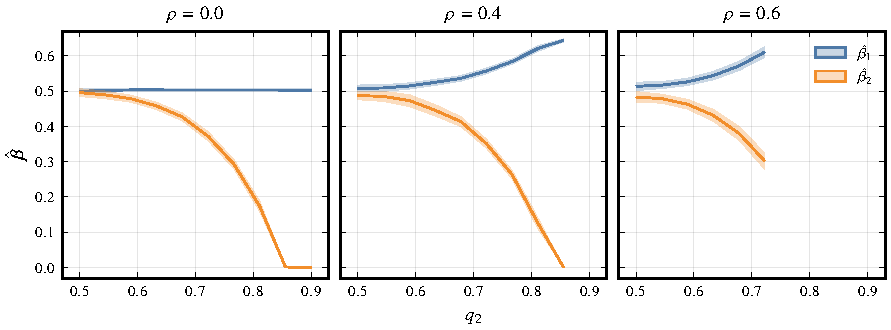
\includegraphics[]{orthogonality.pdf}
  \caption{%
    Estimates of the regression coefficients from the lasso,
    \(\hat{\vec{\beta}}\), for the two features in the experiment in
    \Cref{sec:orthogonality-assumption}. The first feature is binary with class
    balance \(q_1 = 0.5\) and the second is binary with class balance \(q_2 \in [0.5, 0.9]\).
    The features are correlated with correlation \(\rho\). The plot shows means and
    95\% normal confidence intervals averaged over 100 iterations. Note
    that it's impossible to achieve high levels of correlation when the second
    feature is highly imbalanced, which is why the results for \(\rho = 0.4\) and \(0.6\)
    do not cover the whole range of \(q_2\) values.
  }
  \label{fig:orthogonality}
\end{figure}

\begin{theorem}[Correlation for Dichotomized Normal Variables]
  Let \(X\) and \(Y\) be two standard normal random variables with correlation \(\rho\).
  Define \(Z = \bm{1}[Y > \alpha]\) where \(\alpha = \cdf^{-1}(q)\) is the
  quantile at which \(Y\) is dichotomized.
  Then
  \[
    \cor(X,Z)
    = \frac{\rho\pdf(\alpha)}{\sqrt{q \bigl(1 - q\bigr)}} \rightarrow 0 \quad\text{as}\quad q \rightarrow 1
  \]
\end{theorem}
\begin{proof}
  Let \(Z = \mathbf{1}[Y > \alpha]\) with \(\alpha = \cdf^{-1}(q)\). Then,
  using the law of total expectation, we have
  \[
    \E(XZ) = \E\bigl(\E(XZ \mid Y)\bigr) = \E\bigl(\rho Y \bm{1}[Y > \alpha]\bigr)
    = \rho \int_{\alpha}^{\infty} y \pdf(y)\,\du y = \rho \pdf(\alpha).
  \]
  Since \(\var(X) = 1\) and \(\var(Z) = q (1 - q)\), it follows that
  \[
    \cor(X,Z) = \frac{\E(XZ)}{\sqrt{\var(X)\,\var(Z)}} = \frac{\rho \pdf(\alpha)}{\sqrt{q \bigl(1 - q\bigr)}}.
  \]
  And since \(\pdf(\alpha) \to 0\) exponentially fast as \(q \to 1\), it follows that
  \(\cor(X,Z) \to 0\) as \(q \to 1\).
\end{proof}

\begin{theorem}[Correlation with Bernoulli Variable]
  Let \(X\) be a continuous random variable and \(Y\) be a Bernoulli random variable defined as:
  \[
    Y = \begin{cases}
      1 & \text{with probability } p,   \\
      0 & \text{with probability } 1-p.
    \end{cases}
  \]
  Let \(\mu_1 = \E \left( X \mid Y=1 \right)\), \(\mu_0 = \E \left( X \mid Y=0 \right)\) and
  $\sigma_X^2 = V \left(X \right)$ Then the correlation between \(X\) and \(Y\) is given by:
  \[
    \rho_{X,Y} = \frac{(\mu_1 - \mu_0)}{\sigma_X}\sqrt{p(1-p)}.
  \]
\end{theorem}

\begin{proof}
  The correlation \(\rho_{X,Y}\) is defined as:
  \[
    \rho_{X,Y} = \frac{\mathrm{Cov}(X,Y)}{\sqrt{\mathrm{Var}(X)\mathrm{Var}(Y)}}.
  \]
  We have \(\mathrm{Var}(Y)=p(1-p)\). Using the law of total covariance:
  \begin{align*}
    \mathrm{Cov}(X,Y) & = \E (XY) - \E(X) \E(Y)           \\
                      & = p\mu_1 - (p\mu_1 + (1-p)\mu_0)p \\
                      & = p(1-p)(\mu_1 - \mu_0).
  \end{align*}
  Since $\Var (Y)=p(1-p)$ the result follows.
\end{proof}

\begin{corollary}[Gaussian-Bernoulli Case]
  Suppose \(X\) and \(Z\) are jointly Gaussian random variables with:
  \[
    X, Z \sim N(0,1), \quad \mathrm{Corr}(X,Z)=\rho,
  \]
  and define \(Y=\mathbf{1}[Z>\alpha]\). Then the correlation between \(X\) and \(Y\) is:
  \[
    \rho_{X,Y} = \frac{\rho\,\phi(\alpha)}{\sqrt{\Phi(\alpha)(1 - \Phi(\alpha))}},
  \]
  where \(\phi(\alpha)\) and \(\Phi(\alpha)\) are the PDF and CDF of the standard normal
  distribution, respectively. Further for \(q = \Phi(\alpha)\), we have: $$ \rho_{X,Y} \to 0
    \quad \text{as} \quad q \to 1. $$
\end{corollary}

\begin{proof}
  From the theorem above, we identify:
  \begin{itemize}
    \item \(p = P(Z>\alpha) = 1-\Phi(\alpha)\).
    \item Since \((X,Z)\) is jointly normal, \(X|Z=z \sim N(\rho z, 1-\rho^2)\), we have:
          \[
            \mu_1 = E[X \mid Z>\alpha] = \rho E[Z \mid Z>\alpha] = \rho \frac{\phi(\alpha)}{1-\Phi(\alpha)}.
          \]
    \item Similarly,
          \[
            \mu_0 = E[X \mid Z \leq \alpha] = \rho E[Z \mid Z\leq\alpha] = -\rho\frac{\phi(\alpha)}{\Phi(\alpha)}.
          \]
  \end{itemize}
  Thus:
  \[
    \mu_1 - \mu_0 = \rho\left(\frac{\phi(\alpha)}{1-\Phi(\alpha)} + \frac{\phi(\alpha)}{\Phi(\alpha)}\right) = \frac{\rho\phi(\alpha)}{\Phi(\alpha)(1-\Phi(\alpha))}.
  \]
  Substituting these results into the theorem, we obtain:
  \begin{align*}
    \rho_{X,Y} & = \frac{\rho\phi(\alpha)}{\Phi(\alpha)(1-\Phi(\alpha))}\sqrt{\Phi(\alpha)(1-\Phi(\alpha))} \\[6pt]
               & = \frac{\rho\,\phi(\alpha)}{\sqrt{\Phi(\alpha)(1 - \Phi(\alpha))}}.
  \end{align*}
  Finally, note that $\rho(\alpha)$ is bounded hence $\rho_{X,Y} \rightarrow 0 $ as $q=\Phi(\alpha) \rightarrow 0$.
\end{proof}

One can also compute bounds for two correlated Bernoulli variables: Let \(X \sim
\mathrm{Bernoulli}(p)\) and \(Y \sim \mathrm{Bernoulli}(q)\) with \(0 < p,q < 1\). Their
correlation coefficient is given by
\[
  \rho = \frac{P(X=1,Y=1)-pq}{\sqrt{p(1-p)q(1-q)}},
\]
where the joint probability \(P(X=1,Y=1)\) satisfies the Fréchet bounds:
\[
  \max\{0,\, p+q-1\} \le P(X=1,Y=1) \le \min\{p,\, q\}.
\]
Thus, the extreme values of \(\rho\) are:
\[
  \rho_{\max}(p,q) = \frac{\min\{p,q\}-pq}{\sqrt{p(1-p)q(1-q)}}
\]
and
\[
  \rho_{\min}(p,q) = \frac{\max\{0,\, p+q-1\}-pq}{\sqrt{p(1-p)q(1-q)}}.
\]

